\documentclass{edm_template}

%\usepackage{amsthm,amsmath,amsfonts}
\usepackage{bm}
\usepackage{comment}

\newcommand{\yti}{y_{Ti}}
\newcommand{\yci}{y_{Ci}}
\newcommand{\yhati}{\hat{y}_{Ci}}
\newcommand{\yhat}{\hat{y}_C}
\newcommand{\tauhat}{\hat{\tau}}
\newcommand{\rebar}{\hat{\tau}_{rebar}}
\newcommand{\model}{\hat{y}_0(\cdot)}
\newcommand{\pred}{\hat{y}_0(\bm{x})}
\newcommand{\predi}{\hat{y}_0(\bm{x}_i)}
\newcommand{\EE}{\mathbb{E}}

\newtheorem{prop}{Proposition}


\begin{document}

\title{Using Big Data to Sharpen Design-Based Inference in A/B Tests}

\numberofauthors{4} 
\author{
% 1st. author
\alignauthor Adam C Sales\\
       \affaddr{University of Texas at Austin}\\
       \affaddr{536C George I. S\'{a}nchez Building}\\
       \affaddr{Austin, TX 78705}\\
       \email{asales@utexas.edu}
% 2nd. author
\alignauthor Anthony Botelho\\
       \affaddr{Worcester Polytechnic Institute}
       \affaddr{100 Institute Rd}\\
       \affaddr{Worcester, MA 01609}\\
       \email{abotelho@wpi.edu}
% 3rd. author
\alignauthor Thanaporn Patikorn\\
\affaddr{Worcester Polytechnic Institute}
       \affaddr{100 Institute Rd}\\
       \affaddr{Worcester, MA 01609}\\
       \email{tpatikorn@wpi.edu}
\and  % use '\and' if you need 'another row' of author names
% 4th. author
\alignauthor Neil T. Heffernan\\
\affaddr{Worcester Polytechnic Institute}
       \affaddr{100 Institute Rd}\\
       \affaddr{Worcester, MA 01609}\\
       \email{nth@wpi.edu}
}

\maketitle
\begin{abstract}
Randomized A/B tests in educational software are not run in a vacuum: often, reams of historical data are available alongside the data from a randomized trial. This paper proposes a method to use this historical data--often high-dimensional and longitudinal--to improve causal estimates from A/B tests. The method proceeds in two steps: first, fit a machine learning model to the historical data predicting students' outcomes as a function of their covariates. Then, use that model to predict the outcomes of the randomized students in the A/B test. Finally, use design-based methods to estimate the treatment effect in the A/B test, using prediction errors in place of outcomes. This method retains all of the advantages of design-based inference, while, under certain conditions, yielding more precise estimators. This paper will give a theoretical condition under which the method improves precision, and demonstrates it using a deep learning algorithm to help estimate effects in a set of experiments run inside ASSISTments.
% * <neiltheffernaniii@gmail.com> 2018-03-07T16:39:34.243Z:
% 
% What does desing based methods mean? Is that a techincal term?
% 
% ^.
\end{abstract}

\section{Introduction}
Randomized A/B tests hold a lot of promise for the study of student learning within intelligent tutors. 
Not only do they allow for causal inference without fear of confounding, but they also allow for ``design-based'' effect and standard error estimates that are virtually guaranteed to be unbiased \cite{schochet2015statistical}.
These strengths are to the fact that data analysts know exactly how, and with what probability, conditions were assigned to subjects.

The traditional tools for analyzing experiments estimate effects using \emph{only} data from the experiments themselves, discarding data from the ``remnant,'' any (potential) subjects that were not randomized. 
To be sure, this makes good statistical sense: after all, the probabilities of assignment are known only for participants in the experiment, not for the remnant. 
However, data from the remnant may be quite useful---in particular, the extra sample size could improve the precision of experimental effect estimates.
This is especially the case for experiments run within intelligent tutors or other big data environments.
Vast amounts of log data, collected prior to the experiment, in conjuction with powerful machine-learning methods, could help sharpen causal estimates considerably. 

This paper introduces a method for using the remnant in analyzing experiments, without sacrificing any of the benefits of experimentation or making additional modeling assumptions. 
The core of the method is residualization---to predict experimental subjects' outcomes using a model fit to the remnant, and then estimate effects using prediction residuals instead of the outcomes themselves. 
We call the method ``remnant-based residualization,'' or ``rebar.''
Rebar builds on methods suggested in \cite{rosenbaum}, \cite{tame}, and \cite{aronow}. Rebar was first introduced in \cite{salesRebar} as a method to reduce confounding bias in observational studies. 
Here we show that rebar can also improve precision in randomized A/B tests, particularly in educational data mining contexts. 

The next section will formally introduce rebar, and sections \ref{sec:data}, \ref{sec:deepLearning}, and \ref{sec:results} will illustrate it using a deep-learning model to sharpen effect estimates in a set of 22 experiments run within the ASSISTments system \cite{data}. Section \ref{sec:discussion} will conclude. 


\section{Rebar}
\subsection{Experiments and Modeling}
To learn if an intervention worked, or to figure out which of two conditions (say, condition 0 and condition 1) produces better outcomes, statistical models can often be quite helpful. 
To take a common example, analysts might regress an outcome $Y$ on an indicator for condition $Z$, along with a vector of covariates $\bm{x}$.
Then, the estimated coefficient on $Z$ is taken as the estimated effect of condition 1 versus 0, controlling for $\bm{x}$ \cite{yule1899investigation}. 

The shortcomings of this approach are well-known: if the vector $\bm{x}$ is missing a confounder---a covariate that predicts both subjects' choice of condition, 0 or 1, and outcomes $Y$---then the regression estimate will be biased. 
Moreover, even if there are no unmeasured confounders, if the regression model is misspecified, for instance, modeling the relationship between $Y$ and $\bm{x}$ as linear, then the estimate will also be biased. 
On the other hand, a regression model may be run on all available data, producing precise (if inaccurate) estimates. 

Randomized experiments correct regression's faults. 
If subjects are randomly assigned to conditions 0 or 1, then the difference in mean outcomes between the two groups is an unbiased estimate of the average treatment effect.
More precisely, following \cite{neyman} and \cite{rubin}, let $y_{1i}$ be the outcome a subject $i$ \emph{would} experience \emph{if} assigned to condition 1, and let $y_{0i}$ be the outcome $i$ would experience under condition 0.
Then $\bar{y}_1$ is the average outcome that would have occurred had everyone in the experiment been assigned to 1, and $\bar{y}_0$ is the average outcome had everyone been assigned to 0; Their difference, $\bar{y}_1-\bar{y}_0$, is the ``sample average treatment effect,'' or ATE.
A subject's observed outcome $Y_i=\yti$ if $i$ is assigned to 1, $Z_i=1$; $Y_i=\yci$ if $i$ is assigned to 0. 
(Since observed outcomes $Y$ are a function of $Z$, they are random; we may model potential outcomes $y_0$ and $y_1$ as fixed.)
Assuming one subject's assignment to 1 or 0 doesn't affect anyone else's outcome, then $\tauhat\equiv\bar{Y}_{Z=1}-\bar{Y}_{Z=0}$, the difference in mean outcomes between subjects \emph{actually} assigned to 1, and subjects \emph{actually} assigned to 0, is an unbiased estimate of the ATE.
Since $Z$ is randomized, there are no confounders. 
Since the probability distribution of $Z$ is known exactly, no statistical models, or modeling assumptions, are necessary---the analysis may be ``design-based'' instead of model-based.  
On the other hand, any data from the ``remnant'' of an experiment---the set of subjects outside the experiment, who were not randomized to either condition---must be dropped from the analysis. 
Since subjects in the remnant were not randomized, there is no telling how they may differ from the $Z=0$ or $Z=1$ groups, in ways measured or unmeasured, and there is no telling (exactly, statistically) how their data came to be, so design-based analysis is impossible and any model fit to the remnant is most likely misspecified. 
However, though dropping the remnant from the analysis brings unbiasedness, it also brings a loss of precision---all that sample size, thrown away. 

\subsection{A Role for the Remnant} 
Assume the following setup:
a set of users, ``the experimental set'' were randomized to either condition 0 or condition 1, and their outcomes $\bm{Y}$ were measured at the end of the experiment.
The goal of the experiment is to estimate the ATE, $\bar{y}_1-\bar{y}_0$, the average effect in the experimental set. 
Some more subjects, the remnant, were not randomized; instead, they all received condition 0, the default (this isn't strictly necessary---the theory also works if they received condition 1, a mix of conditions, or something else altogether---but it makes things simpler). 
Outcomes $Y$ were also measured for members of the remnant.
Finally, a set of covariates $\bm{x}$, possibly high-dimensional, of mixed-types, and/or longitudinal, were measured for everyone, in the experimental set and in the remnant. 

Experimental estimates typically drop the remnant, and pay the price of lower precision. 
Instead, we suggest training a machine-learning model on the remnant, and using it to ``residualize" the data from the experimental set; we call this algorithm ``remnant-based residualization'' or ``rebar.''
The process is as follows:
\begin{enumerate}
 \item Using data from the remnant, train a model $\model$ to predict $y_0$ as a function of $\bm{x}$.
 \item Validate $\model$ (using cross-validation or other techniques). if it performs well, proceed; otherwise return to step 1, choosing a different model.
 \item Use $\model$ and covariates $\bm{x}$ in the experimental set to generate predicted outcomes $\pred$ and residuals, $e=Y-\pred$.
 \item Estimate the ATE as a difference in mean residuals, $\rebar=\bar{e}_{Z=1}-\bar{e}_{Z=0}$
\end{enumerate}
Just like the traditional estimator $\tauhat$, the rebar estimator $\rebar$ is design-based---its logical basis is the designed experiment, not a model. 
On the other hand, it harvests information from the remnant to improve upon $\tauhat$.

Rebar works because the predictions $\pred$ were generated from an external sample---the remnant---and pre-treatment covariates $\bm{x}$.
Subject $i$'s prediction $\predi$ will be the same whether $i$ is assigned to 0 or to 1.
Since there's no treatment effect on $\pred$, subtracting $\pred$ from $Y$ only removes noise---not part of the treatment effect. 
When treatment is randomized, $Z$ is independent of $\pred$, so, in expectation, the mean of $\pred$ will be equal across the two treatment groups.
  In fact, the rebar estimator can be re-written as $\rebar=\bar{Y}_{Z=1}-\bar{Y}_{Z=0}-(\overline{\pred}_{Z=1}-\overline{\pred}_{Z=0})$. 
The first term is $\tauhat$, which is unbiased for the ATE. The second term is the difference in means of $\pred$, which is zero in expectation---therefore, $\rebar$ is unbiased. 
This property holds not just for the difference-in-means estimator---rebar can sharpen any treatment effect estimator that is linear in $Y$ and unbiased.

Rebar's main tool is the model $\model$, which predicts $y_C$ as a function of $\bm{x}$. 
In EDM settings, the dimension of available covariates is often very large, and sample sizes are often large as well---machine learning algorithms make strong candidates for $\model$.
$\model$ is not a statistical model \emph{per se}, estimating the parameters of a probability distribution, but as a tool for prediction.
Indeed, it need not be correct in any sense, and its estimates need not be unbiased or consistent. 
Since it is fit on a separate sample from the experimental subjects, the process of fitting it---steps 1 and 2 above---do not affect standard errors, and model misspecification does not lead to bias.

On the other hand, for rebar to be more precise than the usual difference in means, $\model$ must be able to generate decent predictions of $y_C$ in the experimental set. 
This will be the case if $\pred$ is a good prediction of $y_C$---by residualizing, we subtract out the component of $Y$'s variance that is predicted by $\model$. 
In fact, the variance of the rebar estimator is roughly proportionate to the mean-squared prediction error of $\model$, $MSE=||\bm{Y}-\pred||^2/n$, where $n$ is the sample size of the experiment, or, equivalently, the prediction $R^2=1-||Y-\pred||^2/||Y-\bar{Y}||^2$ in the experimental set. 

Since $\model$ is trained in the remnant, its performance in the experimental set (as measured by, e.g. prediction $R^2$) will be hard to gauge at the outset. 
If the distribution of $Y$, conditional on $\bm{x}$, differs widely from the between the two sets, $\model$'s performance may suffer in extrapolation. 
This problem is not fatal: the rebar estimate is unbiased regardless of $\model$'s properties.
However, a model with poor predictive power in the experimental set will not reduce standard errors substantially, and may increase them.
Of course an analyst may calculate $\model$'s $R^2$ in the experimental set, but choosing a model based on $Y$ induces dependence between $Y$ and $\pred$, and may cause bias. 
Models trained on a subset of the remnant that resembles the experimental set---or which weight such a remnant more heavily---may perform better than those trained on the entire remnant. 

The previous discussion assumed simple randomization. 
However, rebar easily extends to more complex designs.
Further, as we will illustrate below, rebar can be extended to regression estimators of causal effects as well, modeling low-dimensional covariates within sample and high-dimensional covariates out of sample. 

\section{Data: 22 Experiments and More}\label{sec:data}
The 22 experiment dataset is a feature-rich dataset on students who participated in randomized controlled trials (RCTs) ran inside a free, online tutoring called ASSISTments \cite{data}. This dataset consists of student-level data from 8,205 unique students participating in 22 A/B tests, 14,947 unique student-RCT pairs in total. 

These RCTs were run within skill builders. Inside ASSISTments, a skill builder is a type of problem set that requires students to practice solving problems until they master the associated skill. Skill mastery is determined by the student's ability to answer a certain number of problems correctly, usually three, in a row.

This feature-rich dataset includes 30 features, including both categorical features, such as student grade levels, and numerical features, such as student performances prior to the experiment. This dataset also includes two dependent measures. The first dependent measure, ``completion,'' is whether the student completed the assignment and achieved mastery. The other dependent measure is the number of problems attempted; for students who achieved mastery, this may be interpreted as mastery speed. The analysis in this paper will focus on the first dependent measure, completion. 



\section{Deep Learning to Predict Completion}\label{sec:deepLearning}
As described in Section 2.1, the model $\model$ is an integral part of the rebar methodology with the purpose of producing predicted outcome $y_0$ as a function of $\bm{x}$. The methodology does not rely on a specific type of model, nor any specific algorithm to be used so long as an estimate for the outcome variable of interest is generated by the model from included covariates. As also stated in that section, the accuracy of the model, however poor, does not lead to bias. That said, models that are more accurate at estimating the outcome variable of interest will likely lead to better estimates of treatment effects.
Deep learning models have been previously applied in educational contexts with promising results, often reporting higher performance over existing methods \cite{piech2015deep}\cite{khajah2016deep}\cite{botelho2017improving}. While the application of such methods is not appropriate to all problem applications due to the size and complexity, the use of such models in this work is justified due to 1) the scale of data available for model training and 2) the inconsequence of producing an uninterpretable model (e.g. the significance and coefficients of individual variables in the model are not intended for study or knowledge discovery). What is needed, again, is simply a prediction model.

We develop and apply a type of deep learning model known as a long short term memory (LSTM) \cite{hochreiter1997long} network. This model is a variant of a recurrent neural network (RNN) \cite{williams1989learning} that is commonly applied to time series data to model temporal relationships within the sequences. The model produces its estimates for each time step by utilizing both covariates provided corresponding to the current time step as well as information from all previous time steps within the series. As such, the model is developed as a sequence-to-sequence method that observes a sequence of student data as input and produces a sequence of outcome estimates of equal length. The model structure utilizes a 3-layer design, with an input layer feeding into a recurrent hidden layer (represented as a layer also connected to itself in previous time steps), before then proceeding to an output layer.

Two separate datasets are used to train and apply the model. The application dataset, comprised of student data from the 22 experiment dataset combined with assignment-level information for all work each student started before beginning the respective experiment. In an attempt to reduce the complexity of the data from which the model must learn, the sequence length of student assignment history is limited such that no more than 10 prior assignments are included for each student. In other words, students who were in a single experiment have a sequence length of 10, with the last time step representing the most recent assignment prior to beginning the experiment. Conversely, students in multiple students may exhibit sequences longer than 10 if participation in the experiments was separated by fewer than 10 assignments. The dataset is comprised of data from 8,297 distinct students and a total of 130,935 student assignments.

The second dataset, used to train and validate the model, is comprised of student data exclusive to that comprising the 22 experiment dataset. Student data, again non-inclusive of students within the 22 experiment dataset, is collected from the non-experimental problem sets found in the application dataset. From these, assignments are randomly sampled, with which the dataset is constructed using the 10 most recent assignments before students begin the sampled assignment. This step, helps to ensure a similar structure of the dataset to that of the application set. Again, for purposes of validity, it is important to stress that no students are found in both the training and application datasets. The dataset contains data from 134,141 distinct students and a total of 686,590 student assignments.

The model uses just 4 assignment-level covariates per time step to predict assignment-level performance on the subsequent assignment. These covariates include the simple measures of completion of the assignment, the number of problems attempted, the number of problems completed, and a measure of inverse mastery speed; this last measure is a transformation of mastery speed, using 1 divided by the number of problems when the assignment was complete, or 0 when the assignment was not completed. While simple in the number of covariates, again, the model also uses information from previous time steps, adding to its complexity (i.e. time step 2 is informed by time step 1, time step 3 is informed by time steps 2 and 1, etc.). The model produces two values per time step corresponding with the desired outcome variable of completion of the next assignment, and also an estimate of inverse mastery speed on the next assignment, using a combined cost of these two measures to update model parameters during training; this second measure was included as it is believed the model may better learn from the data by observing a continuous variable in addition to the binary value of completion and also acts as an example as to how future works may utilize the same methodology to observe beyond the measure of completion presented in this work.

The model is first evaluated using a 5-fold student-level cross-validation. The model is trained for multiple epochs, or training cycles through the data, using a 30\% holdout set, sampled from the training set of each fold, to determine the stopping point of model training; this holdout set also helps stop the model training process before overfitting is detected. It is found that the model produces average AUC of 0.81 and an RMSE of 0.34 for next assignment completion over the 5 folds. Once completed, a final model is trained over the entirety of the training dataset and applied to the application dataset, which has acted as a holdout set during the training and validation process. The next assignment completion estimates, collected from the most recent assignment before students begin each experiment, is then used as the estimated value of completion that is used in subsequent steps of the rebar analyses.


\section{Results}\label{sec:results}

\begin{figure}
\centering
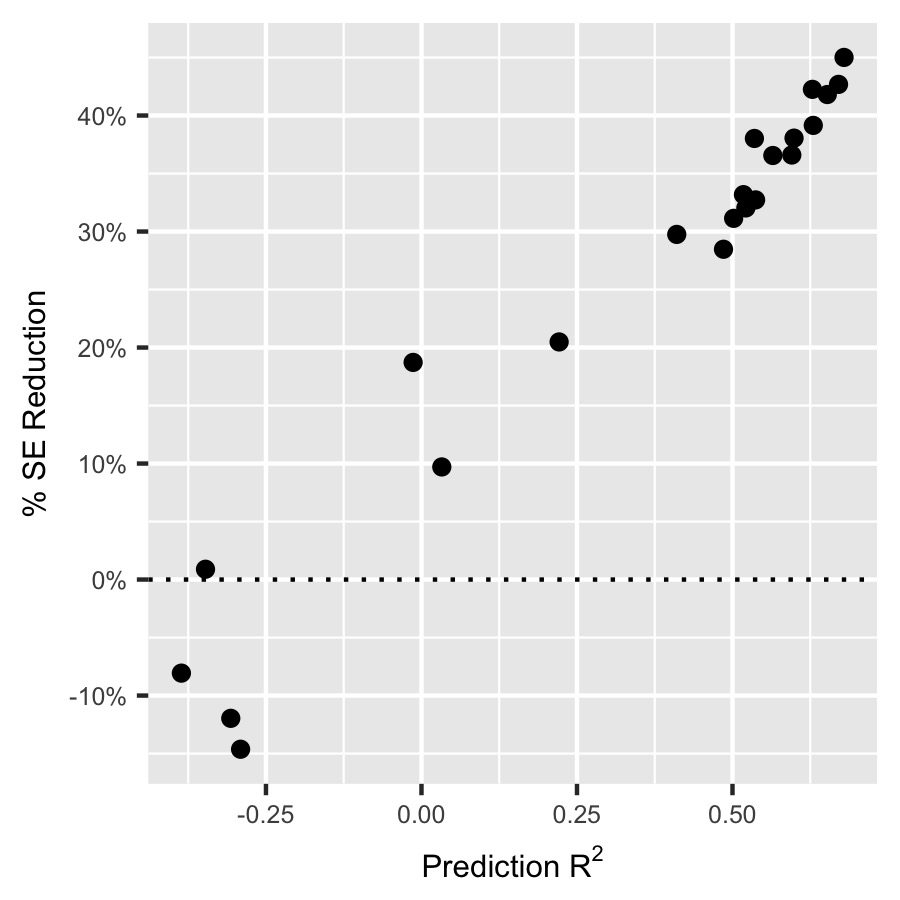
\includegraphics[width=0.5\textwidth]{corVsSE.jpg}
\caption{The improvement in precision of effect estimates as a percentage of the usual precision estimate, $[SE(\tauhat)-SE(\rebar)]/SE(\tauhat)$, plotted as a function of $\model$'s prediction $R^2$ in the experimental set.}
\label{fig:r2se}
\end{figure}

We estimated treatment effects of interventions on skill-builder completion for the 22 experiments using both raw outcomes $\bm{Y}$, the usual approach, and using $\bm{e}=\bm{Y}-\bm{\pred}$, the rebar estimator. 
We also estimated standard errors in both cases.
We used difference in means estimators, so the effect estimates are in units of percentage points---how much more likely were students to finish skill builders under the treatment condition than under control. 

Figure \ref{fig:r2se} shows improvement in precision of the rebar estimator over the usual estimator: the difference of the two standard errors, divided by the usual standard error, $(SE_{usual}-SE_{rebar})/SE_{usual}$.
The x-axis shows the prediction $R^2$ of the deep learning model when extrapolated to each of the 22 experimental datasets. 
In 19 of the datasets, the rebar standard errors were lower than the usual standard errors. 
In 15 of those datasets, there was a greater than 25\% improvement, and in four datasets the improvement was greater than 40\%.
The extent of the reduction in standard error corresponded closely to the prediction $R^2$ of $\model$, with the most dramatic improvements occurring when $R^2\gtrsim 0.5$.

\begin{figure}
\centering
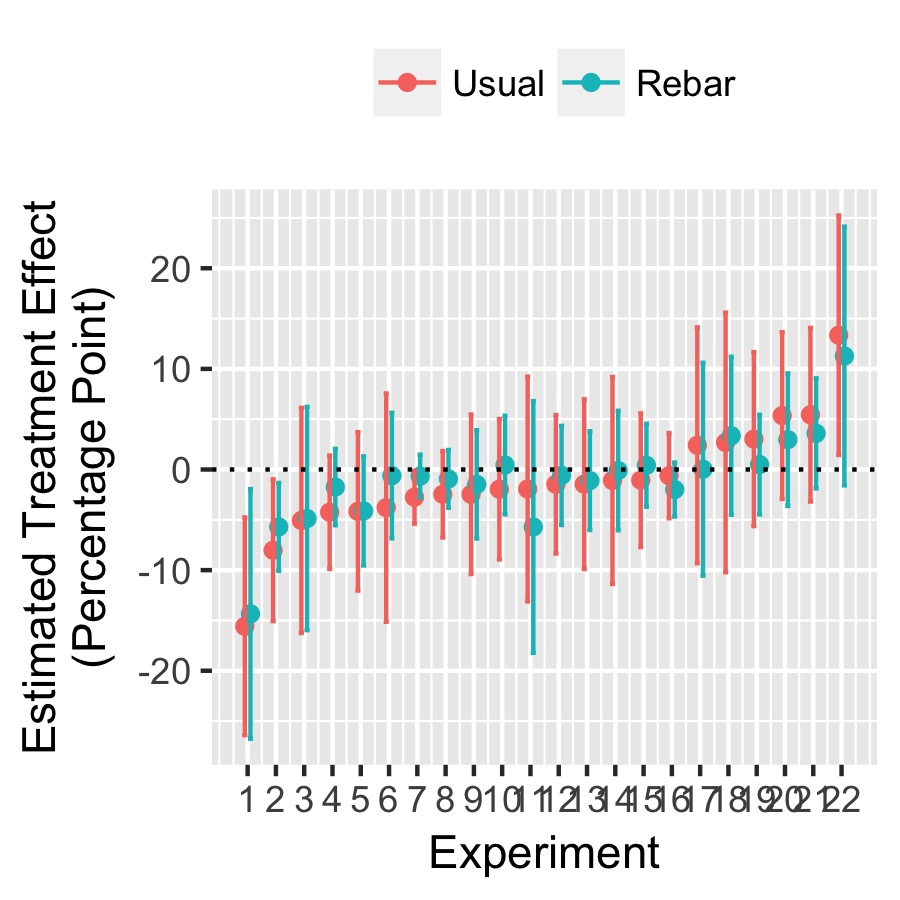
\includegraphics[width=0.5\textwidth]{estEff1.jpg}
\caption{Effect estimates and 95\% confidence intervals for the 22 experiments, using both the usual and rebar estimates. Experiments are ordered by their estimated effect.}
\label{fig:estEff1}
\end{figure}


Figure \ref{fig:estEff1} shows the estimated treatment effects and approximate 95\% confidence intervals (two standard errors in each direction) for the two sets of estimators. 
In all but three cases, the rebar estimate was slightly closer to zero than the usual estimate.
This is what we would expect if most of the true effects were null, so that reducing the noise of the treatment effect estimates would draw them closer to their true values. 
For that reason, although rebar reduced the standard errors in almost all of the experiments, it did not cause any of the non-significant results to become statistically significant. 
In fact, in two cases it had the opposite effect; though this may be disappointing for researchers, it is probably more accurate. 

We also used linear regression to estimate treatment effects, regressing either indicators for completion or prediction errors on indicators for treatment assignment and two covariates: the proportions of students' prior skill builders completed and the proportions of prior skill builder problems students worked that they answered correctly. 
The results, available upon request, are nearly identical.
Although the two covariates improved precision slightly, rebar continued to dominate the usual estimate. 

\begin{comment}
\subsection{Incorporating Regression Controls}
\begin{figure}
\centering
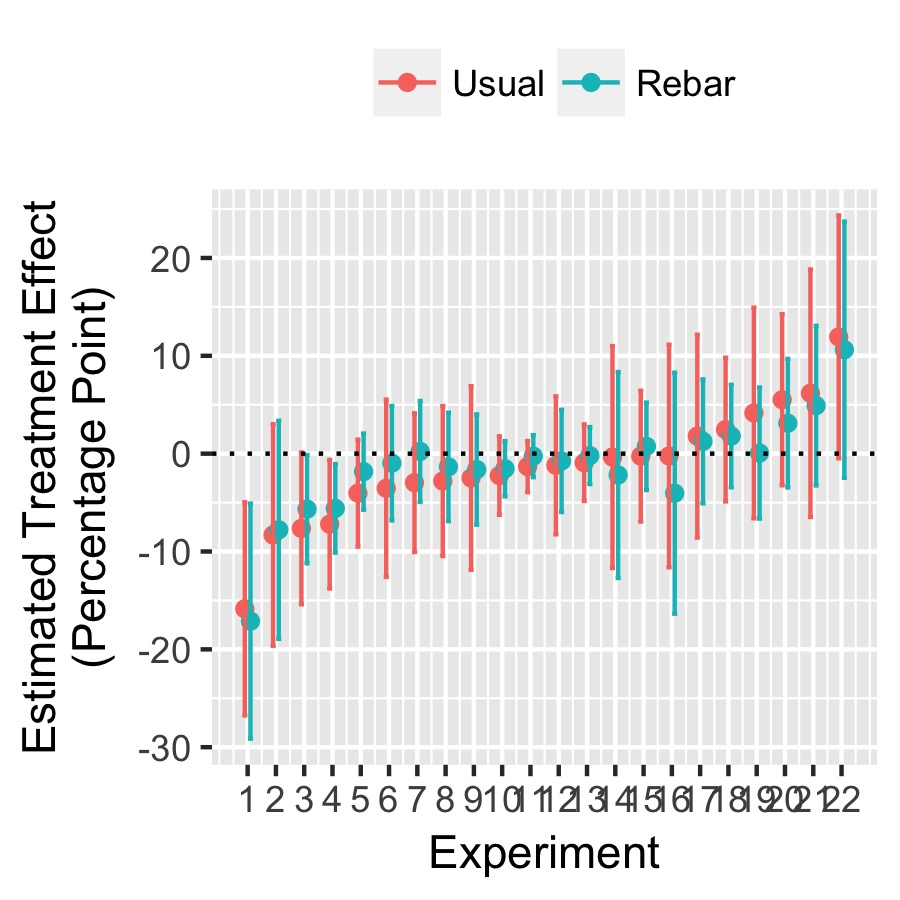
\includegraphics[width=0.5\textwidth]{estEff2.jpg}
\caption{Effect estimates and 95\% confidence intervals for the 22 experiments, from regressions of $Y$ (usual) or $e$ (rebar) on $Z$, prior \% Completed and Prior \% Correct.}
\label{fig:estEff1}
\end{figure}

\begin{figure}
\centering
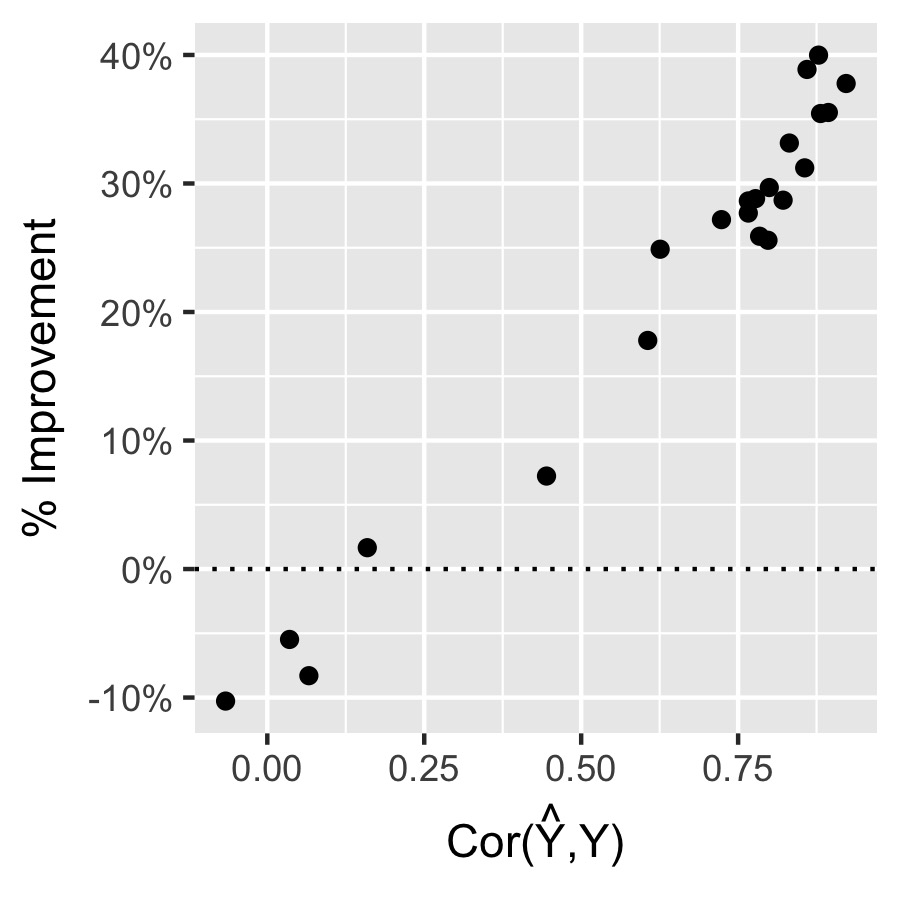
\includegraphics[width=0.5\textwidth]{corVsSE2.jpg}
\caption{The improvement in precision of effect estimates, as a percentage of the usual precision estimate for the usual and rebar regression estimators, plotted as a function of the correlation of outcomes and predictions, $cor(Y,\model{\bm{x}})$.}
\end{figure}
\end{comment}




\section{Discussion}\label{sec:discussion}
The rich, high-dimensional, fine-grained data that educational technology makes available should be a boon to causal inference.
However, big data is subject to the same maladies as small data---confounding from unmeasured variables, and model misspecification.
Classical randomized experiments remain relevant.

The same may not be true for classical design based estimators.
Big data may not be able to correct unmeasured confounding and may exacerbate model misspecification, but we have shown that it can play a significant role reducing the standard errors of treatment effect estimates. 
The method we proposed here retains all of the statistical properties that recommend design-based estimators, while, in most cases, delivering substantially lower standard errors. 
We demonstrated the method's effectiveness using a cutting-edge deep learning algorithm trained to log data from ASSISTments which yielded impressive gains in precision when used to analyze a set of 22 experiments.

Rebar's most important tool in this exercise was the deep learning algorithm, which in 17 of the 22 experiments predicted completion better than the within-sample proportion.
In general, designing prediction algorithms that perform well in the target dataset is the central challenge to effectively implementing rebar. 
Along the same lines, the most important open question is how to design diagnostics for prediction performance that do not rely on ``peeking'' at the experimental outcomes. 
One such diagnostic, termed ``proximal validation,'' was described in \cite{salesRebar}---extending it to experimental studies and showing that it works is the next step in developing this method. 

Wedding classical randomization-based causal inference with modern machine learning and big data can yield unbiased, robust, precise treatment effect estimates in technology-based educational datasets. 

\section{Acknowledgements}
Ben B Hansen provided foundational ideas and valuable guidance in the early stages of this project. This work was funded by a number of Neil's grants.

\bibliographystyle{abbrv}
\bibliography{citations}  
\end{document}
